% !TEX TS-program = pdflatex
% !TEX encoding = UTF-8 Unicode

% This is a simple template for a LaTeX document using the "article" class.
% See "book", "report", "letter" for other types of document.

\documentclass[11pt]{article} % use larger type; default would be 10pt

\usepackage[utf8]{inputenc} % set input encoding (not needed with XeLaTeX)

%%% Examples of Article customizations
% These packages are optional, depending whether you want the features they provide.
% See the LaTeX Companion or other references for full information.

%%% PAGE DIMENSIONS
\usepackage{geometry} % to change the page dimensions
\geometry{a4paper} % or letterpaper (US) or a5paper or....
% \geometry{margin=2in} % for example, change the margins to 2 inches all round
% \geometry{landscape} % set up the page for landscape
%   read geometry.pdf for detailed page layout information

\usepackage{graphicx} % support the \includegraphics command and options\usepackage{graphicx}
\graphicspath{ {images/} }

% \usepackage[parfill]{parskip} % Activate to begin paragraphs with an empty line rather than an indent

%%% PACKAGES
\usepackage{booktabs} % for much better looking tables
\usepackage{array} % for better arrays (eg matrices) in maths
\usepackage{paralist} % very flexible & customisable lists (eg. enumerate/itemize, etc.)
\usepackage{verbatim} % adds environment for commenting out blocks of text & for better verbatim
\usepackage{subfig} % make it possible to include more than one captioned figure/table in a single float
% These packages are all incorporated in the memoir class to one degree or another...

%%% HEADERS & FOOTERS
\usepackage{fancyhdr} % This should be set AFTER setting up the page geometry
\pagestyle{fancy} % options: empty , plain , fancy
\renewcommand{\headrulewidth}{0pt} % customise the layout...
\lhead{}\chead{}\rhead{}
\lfoot{}\cfoot{\thepage}\rfoot{}
\usepackage[]{algorithm2e}

%%% SECTION TITLE APPEARANCE
\usepackage{sectsty}
\allsectionsfont{\sffamily\mdseries\upshape} % (See the fntguide.pdf for font help)
% (This matches ConTeXt defaults)

%%% ToC (table of contents) APPEARANCE
\usepackage[nottoc,notlof,notlot]{tocbibind} % Put the bibliography in the ToC
\usepackage[titles,subfigure]{tocloft} % Alter the style of the Table of Contents
\renewcommand{\cftsecfont}{\rmfamily\mdseries\upshape}
\renewcommand{\cftsecpagefont}{\rmfamily\mdseries\upshape} % No bold!

%%% END Article customizations

%%% The "real" document content comes below...

\title{CS698: Assignment 5}
\author{Ronghao Yang\\ID: 20511920\\Session: 4:00-5:20pm}
%\date{} % Activate to display a given date or no date (if empty),
         % otherwise the current date is printed 

\begin{document}
\maketitle

\section{Exercise 1}
\subsection{Exercise 1.1}
The VGG11 net has been modified for this assignment. The reason is that the original VGG11 net is too complex, our dataset may not need such a complex model. A simplified model may be enough for MNIST dataset. The modified architecture used is the following:\\
\begin{center}
 \begin{tabular}{||c||} 
 \hline
My CNN Net \\ [0.5ex] 
 \hline\hline
 Conv3-64 \\ 
 \hline
  maxpooling \\
 \hline
  Conv3-128 \\
 \hline
maxpooling\\
 \hline
 Conv3-256 \\ 
 \hline
 maxpooling\\
  \hline
  FC-512\\
  \hline
  FC-10\\
  \hline
  soft-max\\
  \hline
\end{tabular}
\end{center}\mbox{}\\
The parameter used are:\\
batch$\_$size = 64\\
learning$\_$rate = 0.01\\
momentum = 0.9\\
epochs = 20\\
In the original question, we are asked why we need to resize the image from 28$\times$28 to 32$\times$32, this reason is the following:\\
In VGG11, there exist 5 maxpooling layers, after each maxpooling layer, the size of the image is reduced by 2 (eg from 32$\times$32 to 16$\times$16), with the image size being 28$\times$28, we are unable to do 5 times of maxpooling.
\subsection{Exercise 1.2}
For this section, the number of epochs is set to be 10.
\paragraph{•test accuracy vs the number of iterations}\mbox{}\\
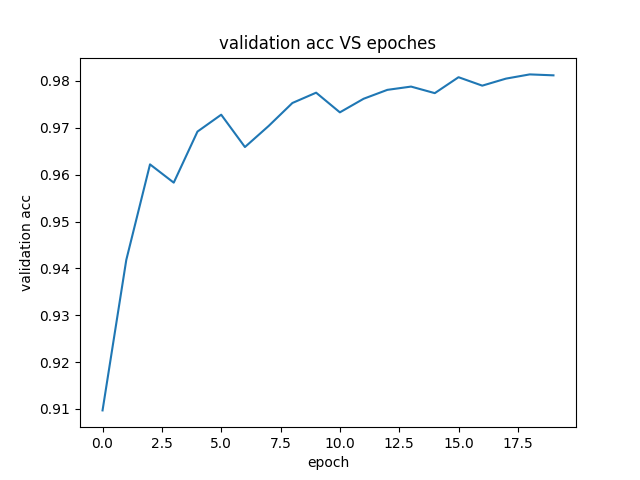
\includegraphics[scale=0.5]{e121.png}
\paragraph{•training accuracy vs the number of iterations}\mbox{}\\
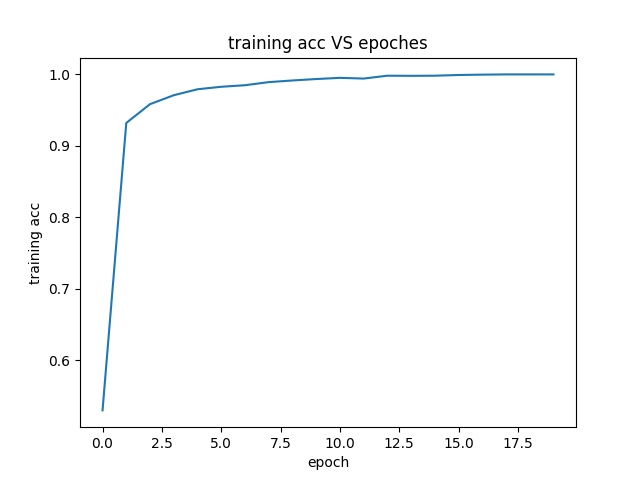
\includegraphics[scale=0.5]{e122.png}
\paragraph{•test loss vs the number of iterations}\mbox{}\\
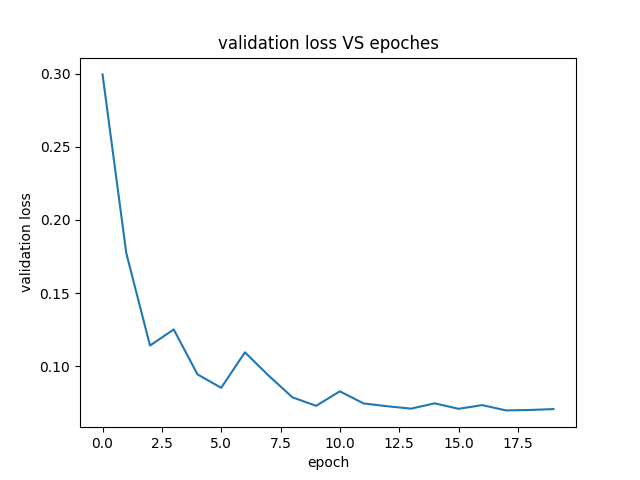
\includegraphics[scale=0.5]{e123.png}
\paragraph{•training loss vs the number of iterations}\mbox{}\\
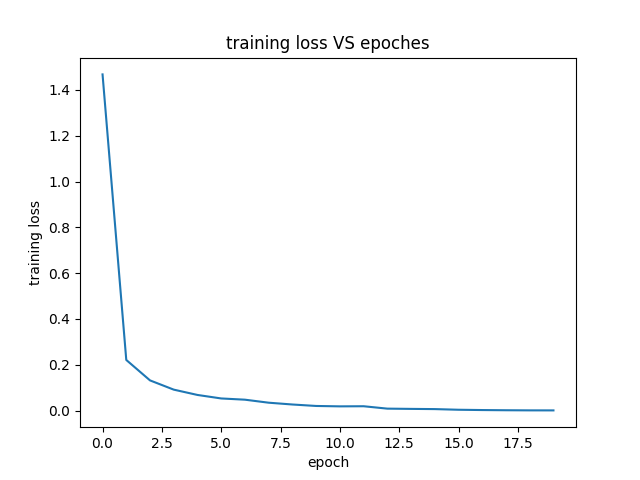
\includegraphics[scale=0.5]{e124.png}
\subsection{Exercise 1.3}
For this section, the number of epochs is set to be 10.
\paragraph{•test accuracy vs the degree of rotation}\mbox{}\\
The more degrees of rotation we apply on the testing set, the lower the testing accuracy is. \\
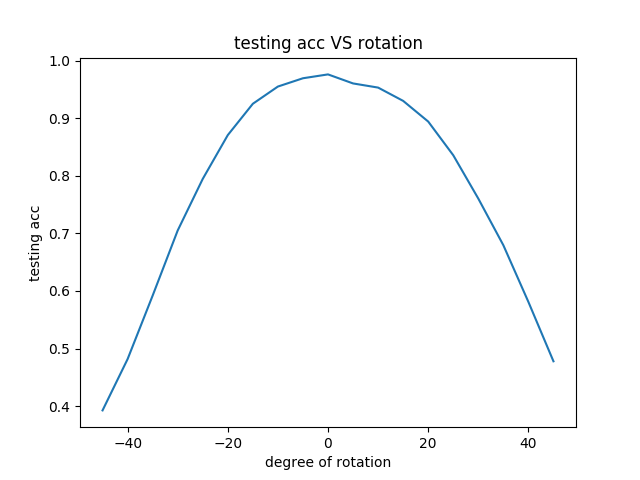
\includegraphics[scale=0.7]{e131.png}
\paragraph{•test accuracy vs Gaussian blurring}\mbox{}\\
The higher radius of Gaussian radius we apply on the testing set, the lower the testing accuracy is.\\
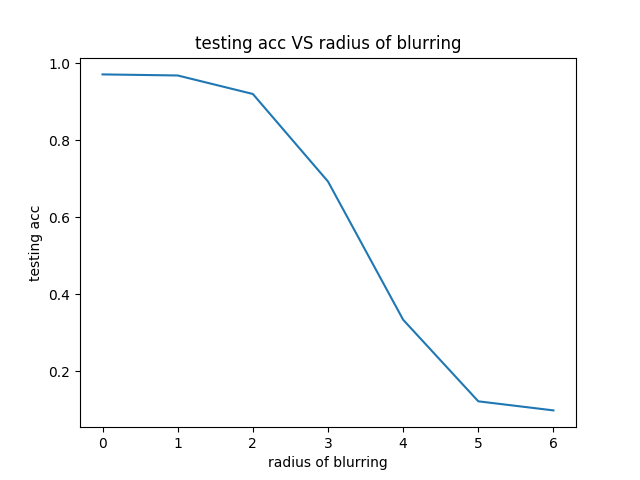
\includegraphics[scale=0.5]{e132.png}

\subsection{Exercise 1.4}
\paragraph{•l2 regularization}\mbox{}\\
As we can see here, with l2 regularization, the overall performance has not been affected much. The accuracy with regularization is slightly lower than the accuracy without regularization, this may comes from the complexity of the model. Our simplified model only has a few layers, adding regularization terms to it makes our model even more simplified.
\subparagraph{•test accuracy vs the number of iterations}\mbox{}\\
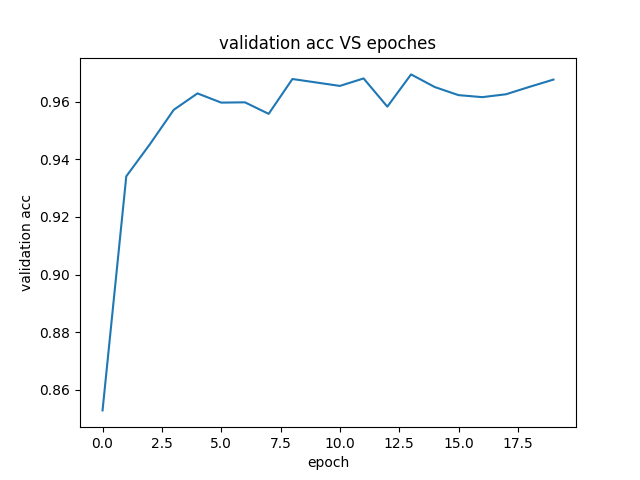
\includegraphics[scale=0.5]{e141val_acc.png}
\subparagraph{•training accuracy vs the number of iterations}\mbox{}\\
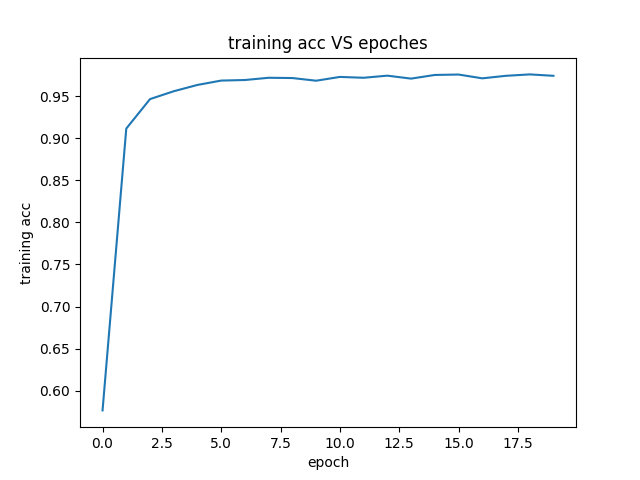
\includegraphics[scale=0.5]{e141train_acc.png}
\subparagraph{•test loss vs the number of iterations}\mbox{}\\
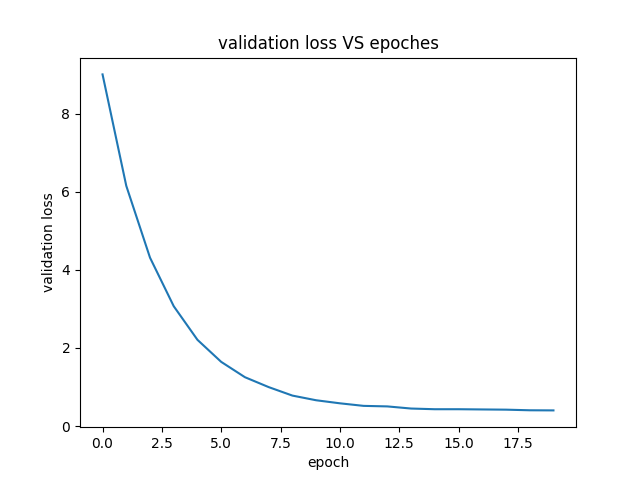
\includegraphics[scale=0.5]{e141val_loss.png}
\subparagraph{•training loss vs the number of iterations}\mbox{}\\
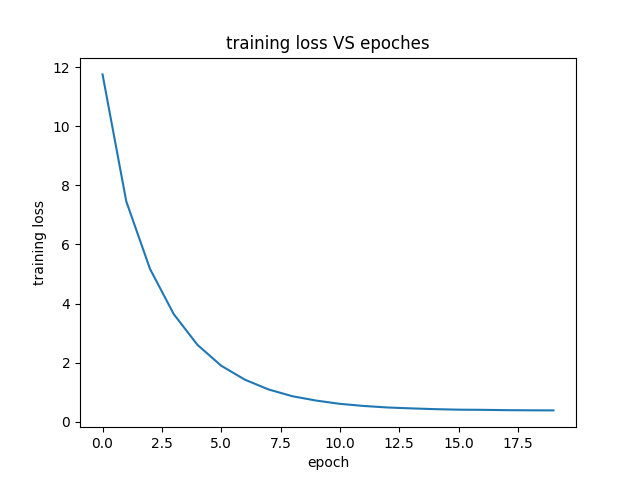
\includegraphics[scale=0.5]{e141train_loss.png}
\subparagraph{•test accuracy vs the degree of rotation}\mbox{}\\
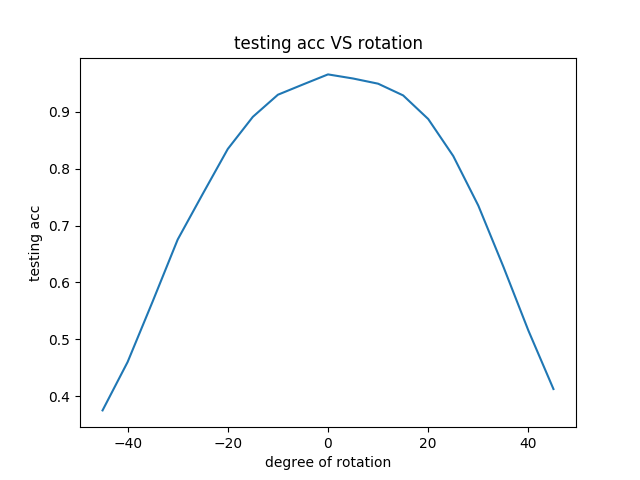
\includegraphics[scale=0.5]{e141rotation.png}
\subparagraph{•test accuracy vs Gaussian blurring}\mbox{}\\
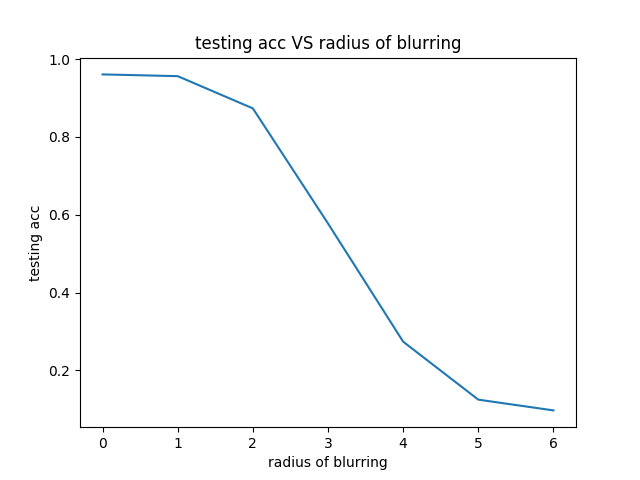
\includegraphics[scale=0.7]{e141blur.png}
\paragraph{•Data augmentation}\mbox{}\\
The original training set has 6000 images, for data augmentation, I have added another 6000*7 additional modified images to it. For those extra 7 batches, the details of the data augmentation are:\\
Batch 1: image rotation -45 degrees\\
Batch 2: image rotation 45 degrees\\
Batch 3: image rotation -25 degrees\\
Batch 4 image rotation 25 degrees\\
Batch 5: image with Gaussian Blur radius = 2\\
Batch 6: image with Gaussian Blur radius = 4\\
Batch 7: image with Gaussian Blur radius = 6\\
With data augmentation, we can see that on the datasets with rotation of Gaussian blurring, the accuracy has significantly increased.\\
In the plots of validation loss and validation accuracy, there exist some huge fluctuations, there might exist some over-fitting problems.
\subparagraph{•test accuracy vs the number of iterations}\mbox{}\\
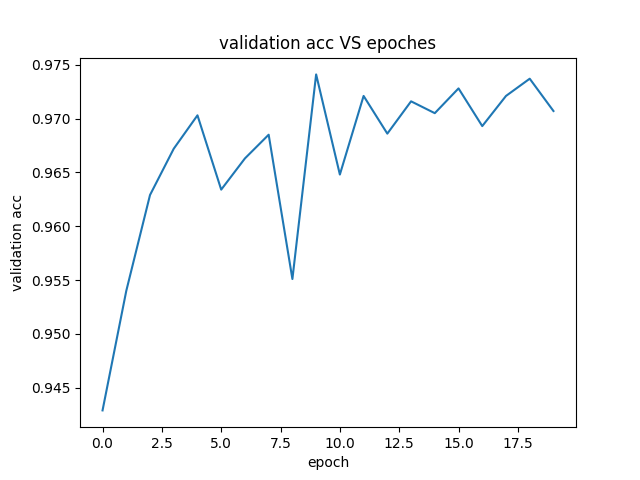
\includegraphics[scale=0.7]{e142val_acc.png}

\subparagraph{•training accuracy vs the number of iterations}\mbox{}\\
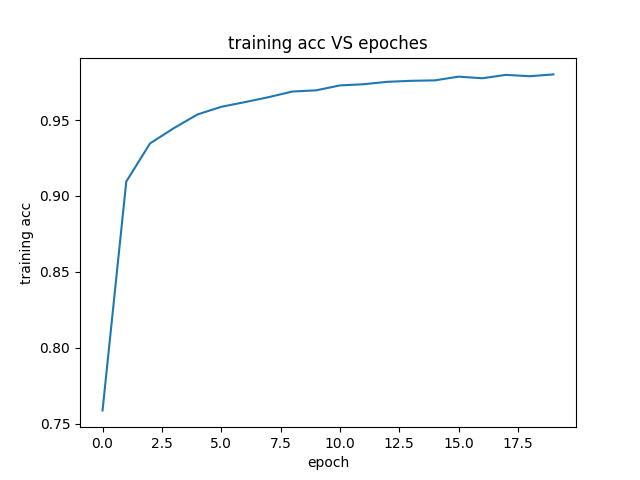
\includegraphics[scale=0.7]{e142train_acc.png}

\subparagraph{•test loss vs the number of iterations}\mbox{}\\
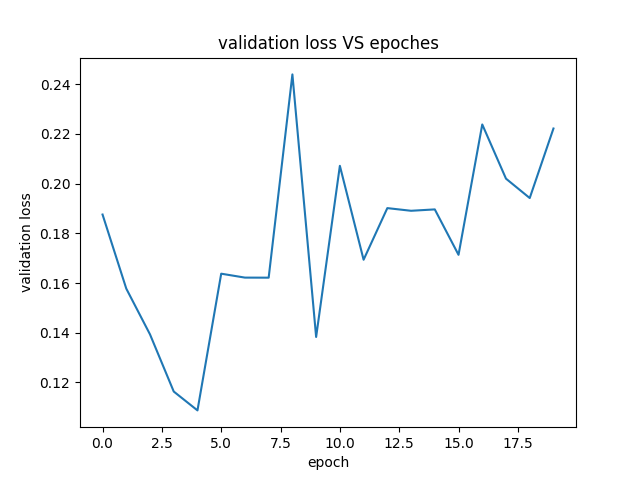
\includegraphics[scale=0.7]{e142val_loss.png}

\subparagraph{•training loss vs the number of iterations}\mbox{}\\
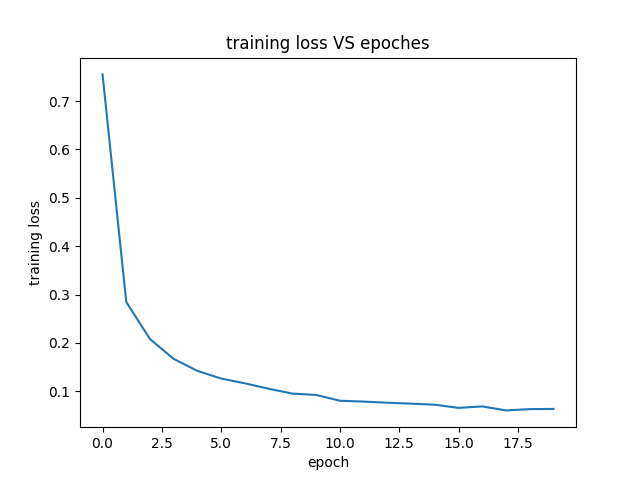
\includegraphics[scale=0.7]{e142train_loss.png}

\subparagraph{•test accuracy vs the degree of rotation}\mbox{}\\
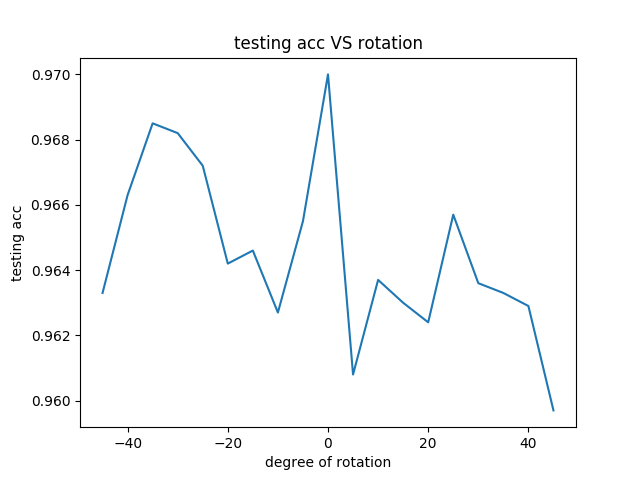
\includegraphics[scale=0.7]{e142rotation.png}

\subparagraph{•test accuracy vs Gaussian blurring}\mbox{}\\
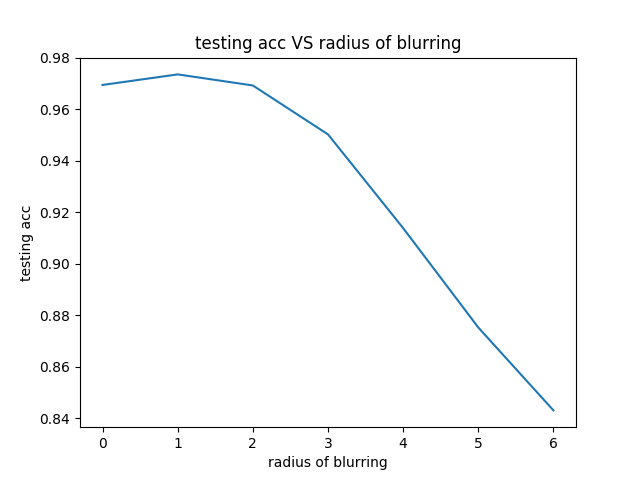
\includegraphics[scale=0.7]{e142blur.png}

\section{Exercise 2}
• When fixing a feature j, we only need  to consider all the values of $X_{ij}$s, since any other thresholds don't make a difference in clustering X into 2 groups. Therefore, only n value are needed to be considered for $t_{j}$s.\\\\ 
• Sorting all $X_{ij}$s takes $nlog(n)$ time.\\\\
• When computing $\mu$ and $\nu$, we set the derivatives of both $\sum_{i:X_{ij}\leq t_{j}}(y_{i}-\mu)^{2}$ and $\sum_{i:X_{ij}> t_{j}}(y_{i}-\nu)^{2}$ to be 0, and calculate the optimal values for $\mu$ and $\nu$. The optimal values are $\mu = \frac{\sum_{i:X_{ij}\leq t_{j}}y_{i}}{n_1}$, $\nu= \frac{\sum_{i:X_{ij}> t_{j}}y_{i}}{n_2}$, where $n_1$ is the number of $y_i$s when $X_{ij}\leq t_{j}$,  $n_2$ is the number of $y_i$s when $X_{ij}> t_{j}$.\\\\
• There are d different features, we need to loop d times.\\\\
• Algorithm that runs in $O(d\;n\;logn)$:\\\\
\begin{algorithm}[H]
\KwData{$X$ $\in$ $R^{n\times d}$, $y \in R^{n}$}
\KwResult{$Jj{best}$, $t_{best}$}
$Loss_{j} = 0$ for all j\\
$T_{j} = 0$ for all j\\
 \For{Feature j \textbf{in} 1...d}{
 $loss_{i}$  = 0 for all i\\
 Sort $X_{:j}$, so that $X_{1j} \leq X_{2j}\leq.... \leq X_{nj}$\\
 Let $S_{1}=0$, $S_{2} = \sum_{k=1}^{i}y_{i}$\\ 
 %Let $T_{1} = 0$, $T_{2} = \sum_{k=1}^{i}y_{i}^{2}$\\
  Let $S_{3} = \sum_{k=1}^{i}y_{i}^{2}$\\
  \For{Threshold $t_{j}$ \textbf{in} $X_{1j}$, $X_{2j}$, ...., $X_{nj}$}{
   %$\mu = \frac{\sum_{i:X_{ij}\leq t_{j}}y_{i}}{n_1}$\;
   %$\nu= \frac{\sum_{i:X_{ij}> t_{j}}y_{i}}{n_2}$\;
   %$loss_{i}$ = $\sum_{i:X_{ij}\leq t_{j}}(y_{i}-\mu)^{2}+\sum_{i:X_{ij}> t_{j}}(y_{i}-\nu)^{2}$
   $S_{1}=S_{1}+y_{i}$, $S_{2}=S_{2}-y_{i}$ when $t_{j} = X_{ij}$\;
   %$T_{1}=T_{1}+y_{i}^2$, $T_{2}=T_{2}-y_{i}^2$ when $t_{j} = X_{ij}$\;
   $loss_{i} = S_{3}-\frac{S_{1}^2}{i}-\frac{S_{2}^2}{n-i}$
   }
   $Loss_{j}$ = min $loss$, for all i\\
   $T_{j}$ = $argmin_{t_{j}}\;loss$
 }
 $j_{best} = argmin_{j}\;Loss$\\
 $t_{best} = T_{J_{best}}$
 \caption{Regression Tree Algorithm}
\end{algorithm}
\end{document}
